\documentclass[a4paper, 12pt]{article}

% Русский язык
\usepackage[T2A]{fontenc}
\usepackage[utf8]{inputenc}
\usepackage[english,russian]{babel}

% Картинки
\usepackage{graphicx}
\graphicspath{{images/}}
\DeclareGraphicsExtensions{.pdf,.png,.jpg}
\usepackage{wrapfig}

% Математика
\usepackage{amsmath,amsfonts,amssymb,amsthm,mathtools} 

% Параметры страницы
\usepackage[left=2cm,right=2cm,top=2cm,bottom=3cm,bindingoffset=0cm]{geometry}

\usepackage{enumitem,xparse}
\usepackage{caption}
\usepackage{subcaption}
\usepackage{float}

\begin{document}

\newgeometry{left=2cm,right=2cm,top=2cm,bottom=1cm,bindingoffset=0cm}
\begin{titlepage}
    
    \begin{center}
        \vspace*{5cm}
        \Huge Московский Физико-Технический Институт
        \vspace*{2cm}\\
        \LARGE Отчет по эксперименту
        \\\vspace*{0.25cm}
        
        \noindent\rule{\textwidth}{1pt}
        \vspace*{-0.25cm}
        
        \huge \textbf{1.1.1\\ Изучение статистических закономерностей на примере измерения фона космического излучения}
        \noindent\rule{\textwidth}{1pt}


       \vfill
        \begin{flushright}
            \begin{minipage}{.4\textwidth}
            \Large Выполнил:\\ Студент 1 курса ФАКТ\\ Группа Б03-504 \\Подмосковнов Лев\\
            \end{minipage}
        \end{flushright}
        
        \vfill
        \normalsize Долгопрудный \\2025
        
    \end{center}
\end{titlepage}
\restoregeometry

\setcounter{page}{2}
\section*{Аннотация}

В работе измеряется удельное сопротивление тонкой проволоки круглого сечения, изготовленной из нихромового сплава. Используются следующие методы измерений сопротивления: 1) определение углового коэффициента наклона зависимости напряжения на проволоке от тока через неё, измеряемых с помощью аналоговых и цифровых вольтметров и амперметров, 2) измерение с помощью моста постоянного тока. Геометрические размеры образца измеряются с помощью линейки, штангенциркуля и микрометра. Детально исследуется систематические и случайные погрешности проводимых измерений.

\section*{Теоретические сведения}

Удельное сопротивление однородной проволоки круглого сечения:

\begin{equation}\label{second}
    \[\rho=R\frac{\pi d^{2}}{4l},\]
\end{equation}


где $R$ -- сопротивление проволоки, $d$ -- её диаметр, $l$ -- длина.

\medskip

\begin{wrapfigure}{r}{6cm}
	\includegraphics[width=6cm]{image.png}
	\caption{\textit{Схема измерения вольт-амперной характеристики проволоки}}
	\label{fig:image}
\end{wrapfigure}

Согласно закону Ома напряжение $V$ и ток $I$ в образце связаны соотношением
\[V=RI.\].

Для измерения напряжения и тока использовалась схема рис. 1

Ввиду неидеальности используемого вольтметра необходимо учесть поправку на его конечное сопротивление $R_{V}$. Показания амперметра $I_{A}$ и вольтметра $V_{B}$ связаны соотношением

\[V_{B}=R'I_{A}\]

\noindentгде $R'$ —- сопротивление параллельно соединенных проволоки и вольтметра, причём $\frac{1}{R'}=\frac{1}{R}+\frac{1}{R_{V}}$, и $R_{V} \gg R,R'$. График зависимости $V_{B}(I_{A})$ должен представлять прямую, угловой коэффициент которой есть $R'$ откуда сопротивление образца может быть найдено как 

\begin{equation}\label{first}
    R=\frac{R_{V}R'}{R_{V}-R'}\approx R'(1+\frac{R'}{R_{V}})
\end{equation}

\section*{Оборудование и инструментальные погрешности}

\textbf{Линейка:} $\Delta_{\text{лин}} = \pm 0,5$ мм (по цене деления). При определении положений контактов имеется дополнительная погрешность, которая может быть оценена как $\Delta_{\text{ЛИН}} \approx \pm 2$ мм

\noindent \textbf{Штангенциркуль:} $\Delta_{\text{ШТ}} = \pm 0,05$ мм (маркировка производителя)

\noindent \textbf{Микрометр:} $\Delta_{\text{МКМ}} = \pm 0,01$ мм (маркировка производителя)

\noindent \textbf{Вольтметр:} Характеристики вольтметра в зависимости от положения переключателя пределов измерения:

\newpage

\begin{tabular}{|l|l|l|}
\hline
Система & Магнито-электрическая \\ \hline
Класс точности & 0.2 \\ \hline
Шкала & линейная, 150 делений \\ \hline
Предел измерений & 0,75 В \\ \hline
Цена деления & 5 мВ \\ \hline
Чувствительность & 150 дел. на 600 мВ \\ \hline
Внутреннее сопротивление & $R_{V} =$ 5 кОм \\ \hline
Погрешность при считывании со шкалы (0,5 цены деления) & $\pm 2 \text{мВ}$ \\ \hline
Макс. погрешность (согласно классу точности) & $\pm 1.2$ мВ (0,2\%) \\ \hline
\end{tabular}

\vspace{1cm}

\noindent \textbf{Амперметр:}

\begin{tabular}{|l|l|l|}
\hline
Система & Цифровая \\ \hline
Предел измерений & 2 А \\ \hline
Разрядность дисплея & 5 ед. \\ \hline
Внутреннее сопротивление & $R_{A}=1,4$ \text{Ом} \\ \hline
Погрешность (при комнатной  & $\Delta_{A}=\pm (0,002 \cdot X + 2k$,  \\
температуре, согласно паспорту прибора) & где $X$ -- измеряемая величина,\\ 
 &  $k$ -- единица младшего разряда ($k=0,01$\text{мА}).  \\ \hline
\end{tabular}

При измерениях в диапазоне от 20 мА до 300 мА погрешность амперметра составила соответственно от $\Delta_{A}$ = ±0,06 мА (0,3\%) до $\Delta_{A}$ = ±0,6 мА (0,2\%).

В диапазоне измерения $R$ от 1 до 10 Ом относительная поправка $\frac{R'}{R_{V}}$ к сопротивлению согласно ф-ле \eqref{first}  составляет от 0,01\% (при $R$ = 1 ом и $R_{V}$ = 10 кОм) до 0,2\% (при $R$ = 10 Ом и $R_{V}$ = 5 кОм). Следовательно, данная поправка заведомо меньше погрешности измерений (0,5\% для вольтметра), поэтому примем далее, что неидеальность вольтметра не оказывает влияния на измерение сопротивления:

\[R \approx R'\]

\noindent \textbf{Мост постоянного тока Р4833:}

Класс точности: 0,1

Разрядность магазина сопротивлений: 5 ед.

Используемый диапазон измерений: $10^{-4}$ – 10 Ом (для множителя $N$ = $10^{-2}$).

Погрешность измерений в используемом диапазоне: ±0,010 Ом

\section*{Результаты измерений и обработка данных}

\subsection*{Измерение диаметра $d$ проволоки.}

\begin{table}[!h]
\begin{center}
\begin{tabular}{|c|c|c|c|c|c|c|c|c|c|c|}
\hline
$N$ изм. & 1 & 2 & 3 & 4 & 5 & 6 & 7 & 8 & 9 & 10 \\ \hline
$d$, мм & 0.37 & 0.37 & 0.36 & 0.37 & 0.36 & 0.37 & 0.37 & 0.36 & 0.36 & 0.36 \\ \hline 
\end{tabular}
\caption{Измерения диаметра проволоки микрометром.}
\end{center}
\end{table}

\clearpage

Среднее значение диаметра: $\overline{d}=\frac{\sum d_i}{N}=0.365$ мм.

Стандартное отклонение: $\sigma_d =\sqrt{\frac{1}{N-1}\sum{(d_i-\overline{d})}^2}=0.0053$ мм.

Случайная погрешность среднего: $\sigma_{\overline{d}}=\frac{\sigma_d}{\sqrt{N}}=0.0017$ мм.

С учётом инструментальной погрешности $\Delta_{\text{мкм}}=0.01$ мм погрешность измерения диаметра может быть вычислена как $\sigma^{\text{полн}}_{\overline{d}}=\sqrt{\sigma^2_{\overline{d}}+\Delta_{\text{мкм}}^2}\approx 0.0101$ мм.

Окончательные результаты измерения диаметра проволоки:

Штангенциркулем: $d=0.4 \pm 0.05$ мм.

Микрометром: $d=0.365 \pm 0.0101$ мм.

\subsection*{Измерение сопротивления проволоки}

Результаты измерений зависимостей показаний вольтметра $V_B$ от показаний амперметра $I_A$ в схеме рис. 1 при разных длинах $l$ образца представлены в табл. 2. Соответствующие графики зависимостей изображены на рис. 2. 

По графику убеждаемся, что экспериментальные данные с хорошей точностью (в пределах инструментальных погрешностей опыта) ложатся на теоретическую прямую $V=RI$, исходящую из начала координат.

Пользуясь методом наименьших квадратов, строим аппроксимирующие прямые $V_B = \overline{R}I$, определяя их угловой коэффициент по формуле

\[\overline{R}=\frac{\langle VI\rangle}{\langle I^2\rangle}\]

\begin{table}[!h]
\begin{center}
\begin{tabular}{|c|c|c|c|c|c|c|c|c|c|c|}
\hline
 & \multicolumn{10}{|c|}{$l=(20.0\pm 0.2)$ см} \\ \hline
$V_B$, мВ & 204 & 260 & 292 & 356 & 620 & 596 & 448 & 292 & 232 & 200 \\ \hline
$I_A$, мА & 100,8 & 129,4 & 144,8 & 177 & 307,3 & 297,9 & 222 & 144,2 & 116 & 99,8 \\ \hline
 & \multicolumn{10}{|c|}{$l=(30.0\pm 0.2)$ см} \\ \hline
$V_B$, мВ & 200 & 228 & 296 & 392 & 584 & 536 & 424 & 320 & 264 & 232 \\ \hline
$I_A$, мА & 66,6 & 76,6 & 99,3 & 130,4 & 194,7 & 177 & 144,3 & 107 & 88 & 77,4 \\ \hline
 & \multicolumn{10}{|c|}{$l=(50.0\pm 0.2)$ см} \\ \hline
$V_B$, мВ & 252 & 376 & 508 & 560 & 592 & 616 & 520 & 432 & 404 & 340 \\ \hline
$I_A$, мА & 50,2 & 74,6 & 101,1 & 111,2 & 117,6 & 122,1 & 103,5 & 85,7 & 80,5 & 67,8 \\ \hline
\end{tabular}
\caption{Зависимость $V_B$ от $I_A$ для разных длин проволоки $l$.}
\end{center}
\end{table}

Случайную погрешность определения углового коэффициента вычисляем как

\[\sigma_R^\text{сл}=\sqrt{\frac{1}{n-1}(\frac{\langle V^2\rangle}{\langle I^2\rangle}-\overline{R}^2}\]
(здесь $n$ = 10 – число точек на графике).

Оценим возможную систематическую погрешность, обусловленную инструментальными
погрешностями приборов. Предполагая, что при всех измерениях относительная погрешность
приборов одинакова, оценим погрешность вычисления частного $R=\frac{V}{I}$ при максимальных
значениях $V$ и $I$:

\[\Delta^{\text{сист}}_R \sim R\sqrt{(\frac{\Delta_V}{V_{max}})^2+(\frac{\Delta_I}{I_{max}})^2}\]

Полная погрешность измерения $R$ не превосходит значения

\[\sigma_R^{\text{полн}} \leq \sqrt{(\sigma_R^\text{сл})^2 + (\Delta^{\text{сист}}_R)^2}\]

Результаты сведены в табл. 3. Там же для сравнения приведены результаты измерения $R$ с помощью моста постоянного тока Р4833 с учётом его погрешности.

\begin{table}[!h]
\begin{center}
\begin{tabular}{|c|c|c|c|c|c|c|c|c|c|c|}
\hline
$l$, см &$\overline{R}$, Ом & $\sigma_R^\text{сл}$, Ом  & $\Delta^{\text{сист}}_R$, Ом & $\sigma_R^{\text{полн}}$, Ом & $R_{\text{мост}}$, Ом \\ \hline
20 & 2.012 & 0.003 & 0.008 & 0.008 & 2.02 $\pm$ 0.01 \\ \hline
30 & 3.01 & 0.009 & 0.012 & 0.015 & 3.013 $\pm$ 0.01 \\ \hline
50 & 5.03 & 0.003 & 0.02 & 0.02 & 5.033 $\pm$ 0.01 \\ \hline
\end{tabular}
\caption{Результаты измерения сопротивления проволоки двумя методами}
\end{center}
\end{table}

Видно, что случайная составляющая измерения сопротивления мала, а основной вклад вносят систематические приборные погрешности. Контрольные измерения с помощью моста дают заниженные результаты, но все отклонения находятся в пределах $\pm \sigma^{\text{полн}}_{R}$.

\subsection*{Вычисление удельного сопротивления}

По формуле \eqref{second} находим удельное сопротивление материала проволоки, используя значения $\overline{R}$. Сравнивая относительные величины погрешностей величин, входящих в \eqref{second}, приходим к выводу, что наибольший вклад в погрешность вносит измерение диаметра проволоки ($2\sigma_d / d \sim 1.4\%$), при этом вкладом остальных измерений можно пренебречь: $\sigma_\rho\approx\frac{2\sigma_d}{d}\rho$

\begin{table}[!h]
\begin{center}
\begin{tabular}{|c|c|c|c|c|c|c|c|c|c|c|}
\hline
N опыта & $\rho, 10^{-6}$ \text{Ом} \cdot \text{м} \\ \hline
1 & $1.052 \pm 0.015$ \\ \hline
2 & $1.049 \pm 0.015$ \\ \hline
3 & $1.052 \pm 0.015$ \\ \hline
\end{tabular}
\end{center}
\end{table}
Усредняя результаты 3-х опытов, окончательно получим:

$\rho=(1.051\pm0.015)\cdot 10^{-6} \text{Ом} \cdot \text{м}$

\newpage

\begin{figure}[h!]
    \centering
    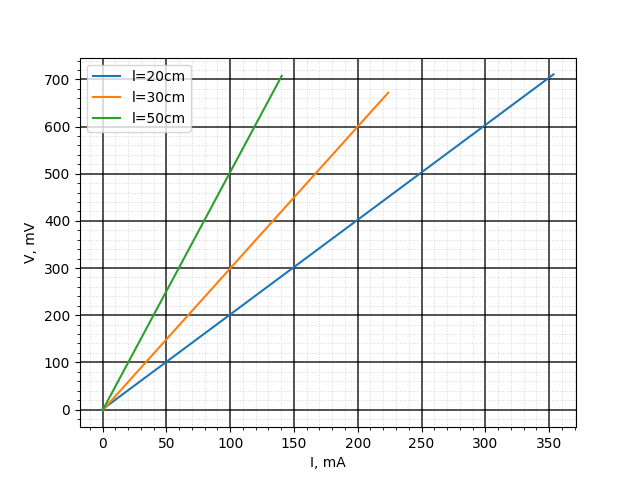
\includegraphics[width=1\textwidth]{g.png}
    \caption{. Результаты измерений напряжения $V_B$ в зависимости от тока $I_A$ для проволок разной длины $l$}
    \label{fig:my_label}
\end{figure}

Для $l=20$ см: k = 2.01 $\pm$ 0.007, b = 0 $\pm$ 1.4

Для $l=30$ см: k = 3.01 $\pm$ 0.003, b = 0 $\pm$ 3.4

Для $l=50$ см: k = 5.05 $\pm$ 0.012, b = 0 $\pm$ 1.14

\section*{Обсуждение результатов и выводы}

В работе получено значение удельного сопротивления образца проволоки из нихромового
сплава с точностью ~1.5\%. Табличные значения для нихрома лежат в диапазоне $\rho_{\text{табл}}= 0,97...1,14 \cdot 10^{-6}$ $\text{Ом} \cdot \text{м}$ в зависимости от состава. Измеренные значения $\rho=(1.051\pm0.015)\cdot 10^{-6} \text{Ом} \cdot \text{м}$ попадают в этот диапазон в пределах одного стандартного отклонения, однако погрешность результата не позволяет определить марку сплава.

Использованный в работе метод измерения сопротивлений позволил получить значения $R$ образцов с довольно высокой точностью образцов с довольно высокой точностью (0,5\%), которая ограничивалась в основном погрешностью аналогового вольтметра. Величина случайной погрешности $\sigma_R^\text{сл}$ показывает, что использование более совершенных измерительных приборов позволило бы довести точность измерения по данной методике до 0,1–0,2\% (при неизменном количестве измерений), что сопоставимо с точностью измерений с помощью мостовой схемы.

Точность измерения удельного сопротивления $\rho$ существенно ограничивается измерением
диаметра проволоки. Поскольку случайная ошибка измерения диаметра оказалась меньше
цены деления прибора (микрометра), уточнение значения диаметра за счет многократных измерений невозможно. По той же причине не удалось проверить, насколько однородной является проволока по сечению.


\end{document}